\documentclass{beamer}

\usepackage[utf8]{inputenc}
\usepackage{hyperref}

\usetheme{Berkeley}
\beamertemplatenavigationsymbolsempty
\setbeamertemplate{headline}{}

\title{Creating a Workflow in FoodChain-Lab 1}
\date{}

\begin{document}
\maketitle

\section{ }

\subsection{Tasks}
\begin{frame}
	\begin{itemize}
		\item Import the Example XLS template to FoodChain-Lab.
		\item You can download it from here: \url{https://github.com/SiLeBAT/BfROpenLabResources/raw/master/GitHubPages/documents/FCL_Example.xlsx}
		\item Via the \textbf{Tracing} node assign weights of "1" to the supermarkets in Hamburg, Karlsruhe, Ingolstadt and Hanover to mark them as outbreak locations.
		\item Use the \textbf{Tracing View} to look at the delivery network.
    \item Use the \textbf{Tracing View} to display the delivery graph in a clearly arranged way.
    \item Apply the \textbf{Default Highlighting} to color the graph.
    \item Visualize the backward and forward trace for an arbitrary station.
	\end{itemize}
\end{frame}

\subsection{1}
\begin{frame}
	\begin{center}
  		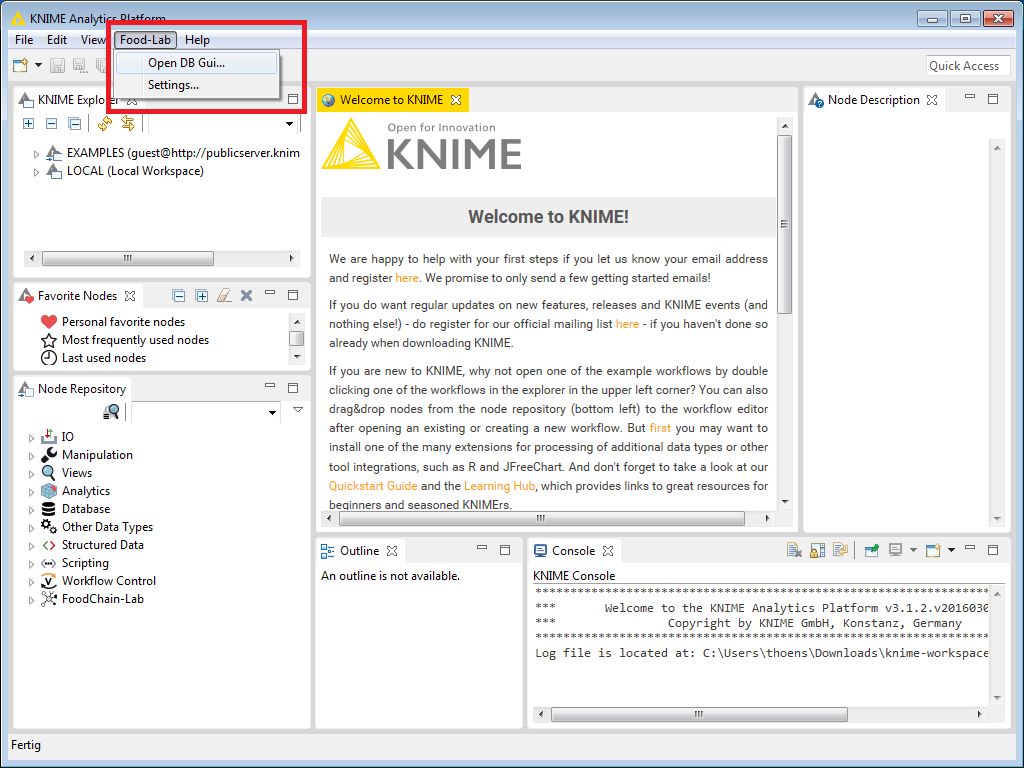
\includegraphics[height=0.6\textheight]{1.png}
	\end{center}
	\begin{itemize}
		\item Select \textbf{Food-Lab $>$ Open DB Gui...} in the menu bar to open the database interface.
	\end{itemize}
\end{frame}

\subsection{2}
\begin{frame}
	\begin{center}
  		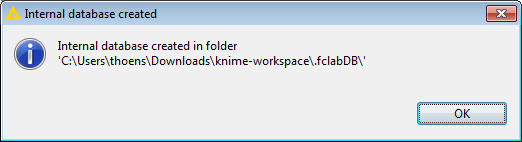
\includegraphics[width=0.9\textwidth]{2.png}
	\end{center}
	\begin{itemize}
		\item If you get a message saying the internal database has been created, click \textbf{OK}.
	\end{itemize}
\end{frame}

\subsection{3}
\begin{frame}
	\begin{center}
  		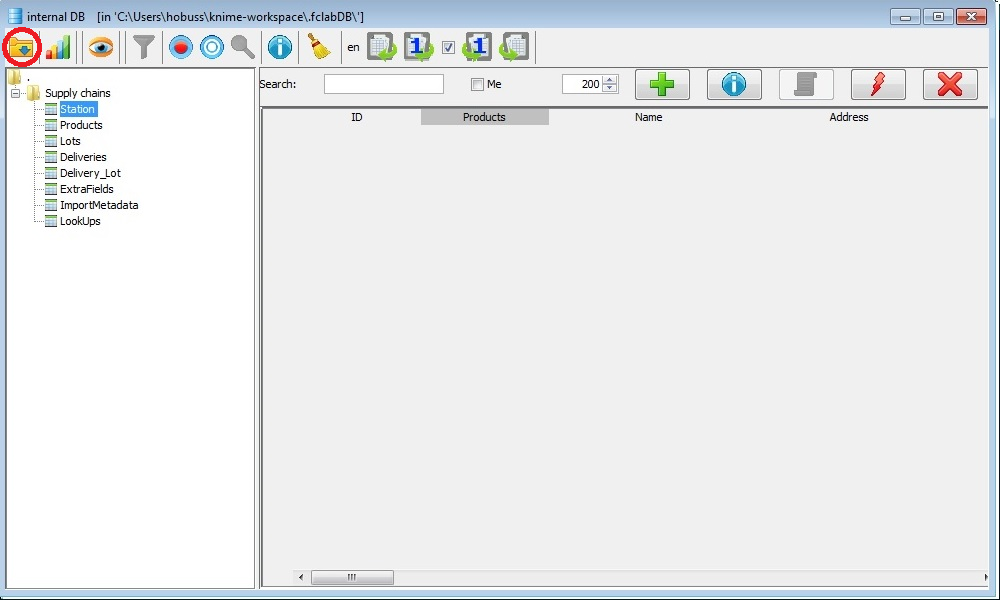
\includegraphics[height=0.6\textheight]{3.png}
	\end{center}
	\begin{itemize}
		\item In the database interface click the \textbf{Table import} button in the upper left corner.
	\end{itemize}
\end{frame}

\subsection{4}
\begin{frame}
	\begin{center}
  		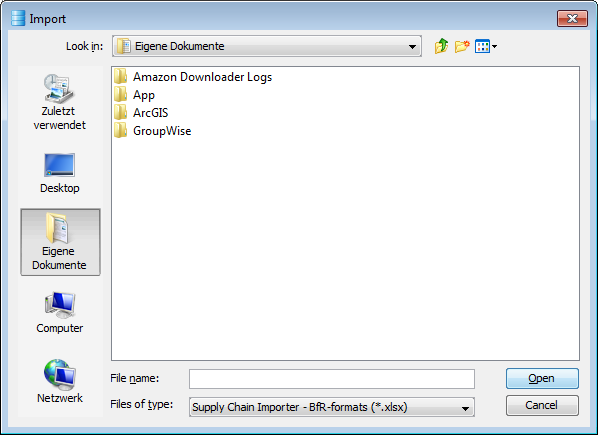
\includegraphics[height=0.6\textheight]{4.png}
	\end{center}
	\begin{itemize}
		\item Now a file dialog will pop up.
		\item *.xlsx files in FoodChain-Lab format can be selected here.
	\end{itemize}
\end{frame}

\subsection{5}
\begin{frame}
	\begin{center}
  		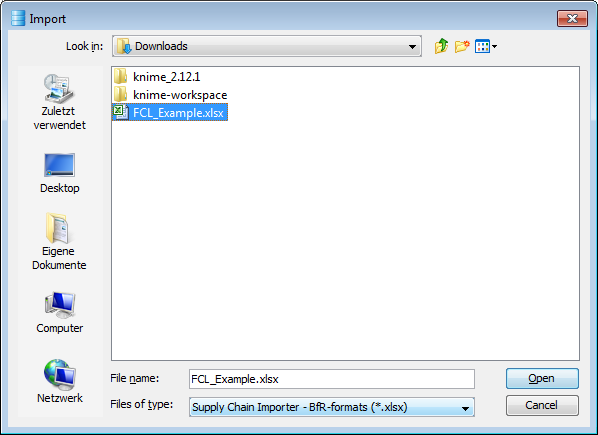
\includegraphics[height=0.6\textheight]{5.png}
	\end{center}
	\begin{itemize}
		\item Download the example file from \url{https://github.com/SiLeBAT/BfROpenLabResources/raw/master/GitHubPages/documents/FCL_Example.xlsx}.
		\item Select the file in the dialog and press \textbf{Open}.
	\end{itemize}
\end{frame}

\subsection{6}
\begin{frame}
	\begin{center}
  		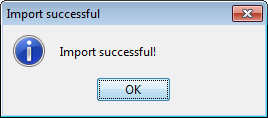
\includegraphics[width=0.5\textwidth]{6.png}
	\end{center}
	\begin{itemize}
		\item When the importing is finished you see a dialog with errors/warnings, that occurred in the import process.
		\item No errors ocurred, so just press \textbf{OK}.
	\end{itemize}
\end{frame}

\subsection{7}
\begin{frame}
	\begin{center}
  		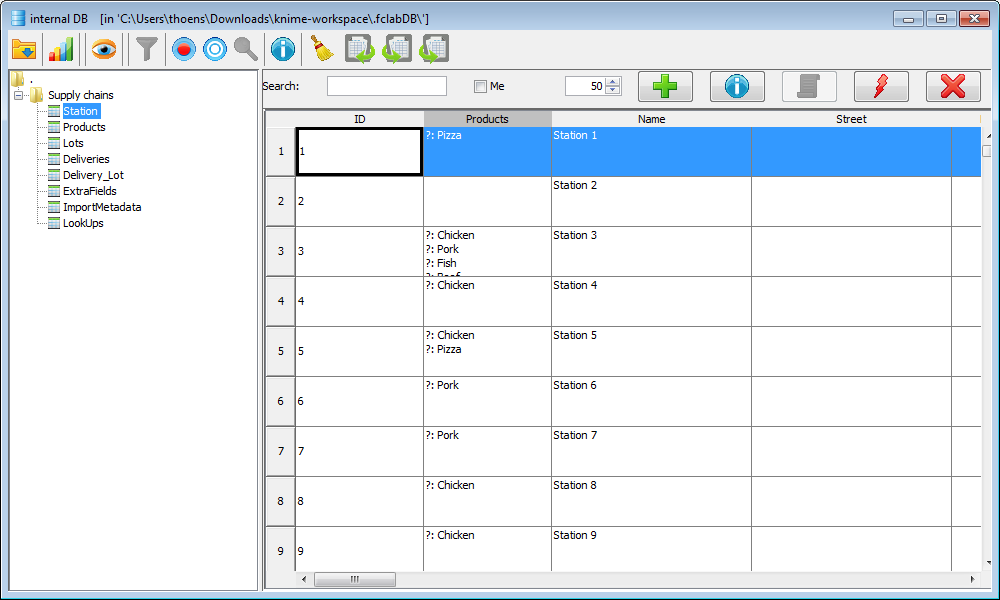
\includegraphics[height=0.6\textheight]{7.png}
	\end{center}
	\begin{itemize}
		\item In the database interface, you can now look at the imported data and check the data for duplicates.
		\item Close the dialog.
	\end{itemize}
\end{frame}

\subsection{8}
\begin{frame}
	\begin{center}
  		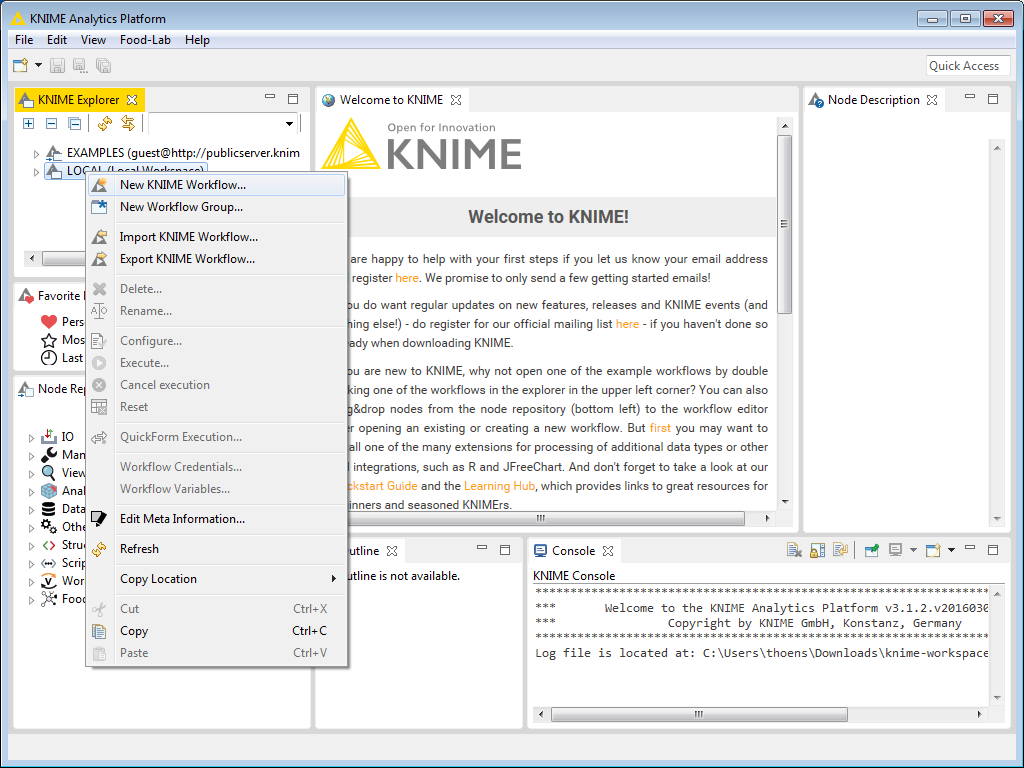
\includegraphics[height=0.6\textheight]{8.png}
	\end{center}
	\begin{itemize}
		\item Now we want to create a workflow, that uses the imported data.
		\item Right click on \textbf{LOCAL} in the \textbf{KNIME Explorer} and select \textbf{New KNIME Workflow...}
	\end{itemize}
\end{frame}

\subsection{9}
\begin{frame}
	\begin{center}
  		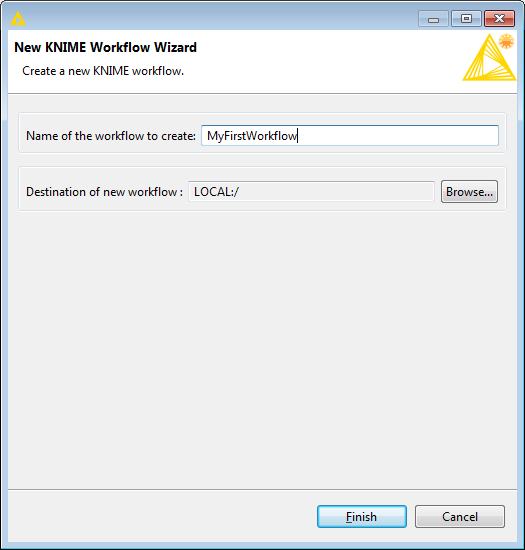
\includegraphics[height=0.6\textheight]{9.png}
	\end{center}
	\begin{itemize}
		\item In the dialog set the name of the workflow to "MyFirstWorkflow" and click \textbf{Finish}.
	\end{itemize}
\end{frame}

\subsection{10}
\begin{frame}
	\begin{center}
  		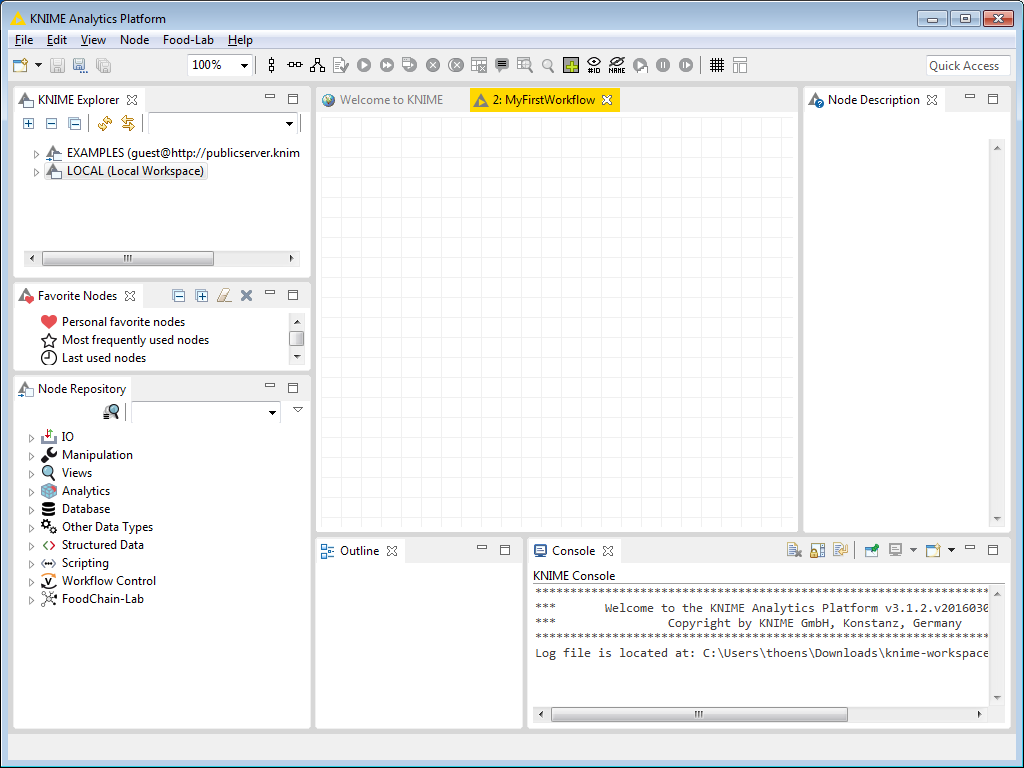
\includegraphics[height=0.6\textheight]{10.png}
	\end{center}
	\begin{itemize}
		\item The created workflow will be shown in the editor in the center.
	\end{itemize}
\end{frame}

\subsection{11}
\begin{frame}
	\begin{center}
  		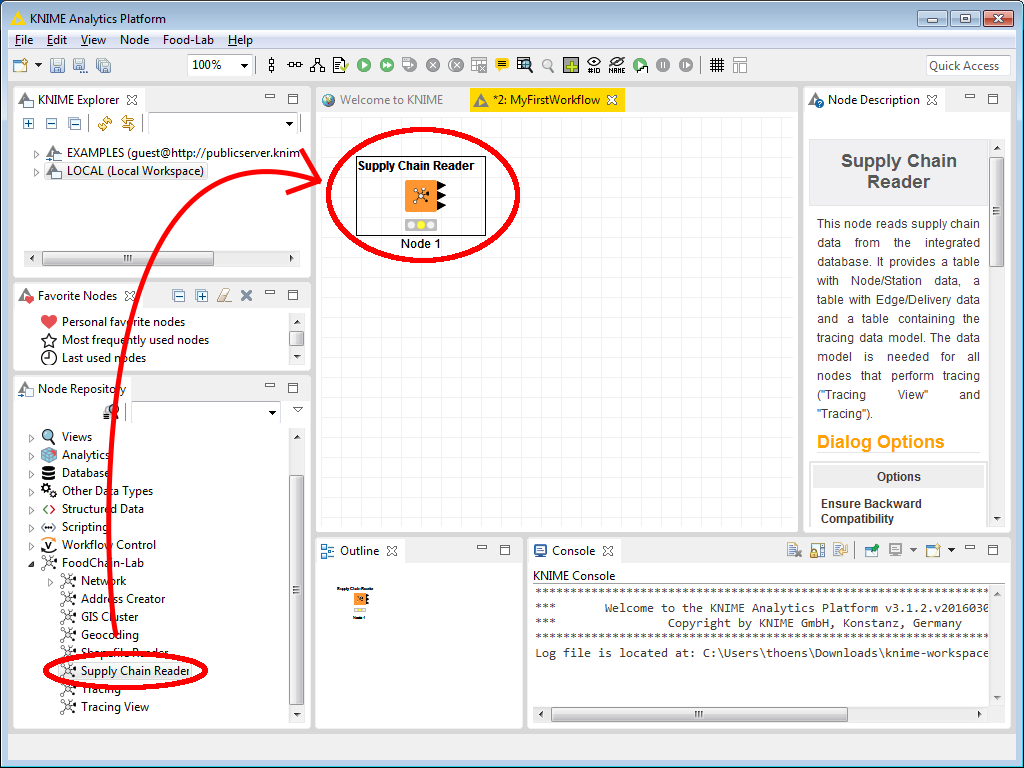
\includegraphics[height=0.6\textheight]{11.png}
	\end{center}
	\begin{itemize}
		\item Drag the \textbf{Supply Chain Reader} from the \textbf{Node Repository} to the workflow.
	\end{itemize}
\end{frame}

\subsection{12}
\begin{frame}
	\begin{center}
  		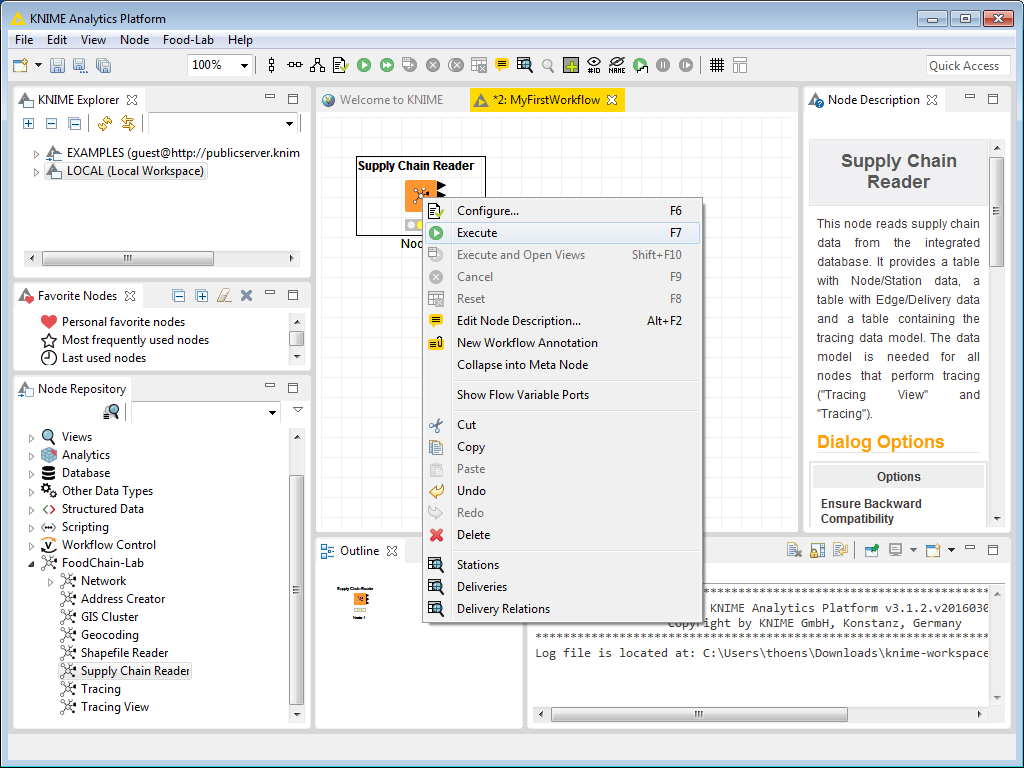
\includegraphics[height=0.6\textheight]{12.png}
	\end{center}
	\begin{itemize}
		\item We do not need to configure the \textbf{Supply Chain Reader}.
		\item Right click on it and select \textbf{Execute}.
	\end{itemize}
\end{frame}

\subsection{13}
\begin{frame}
	\begin{center}
  		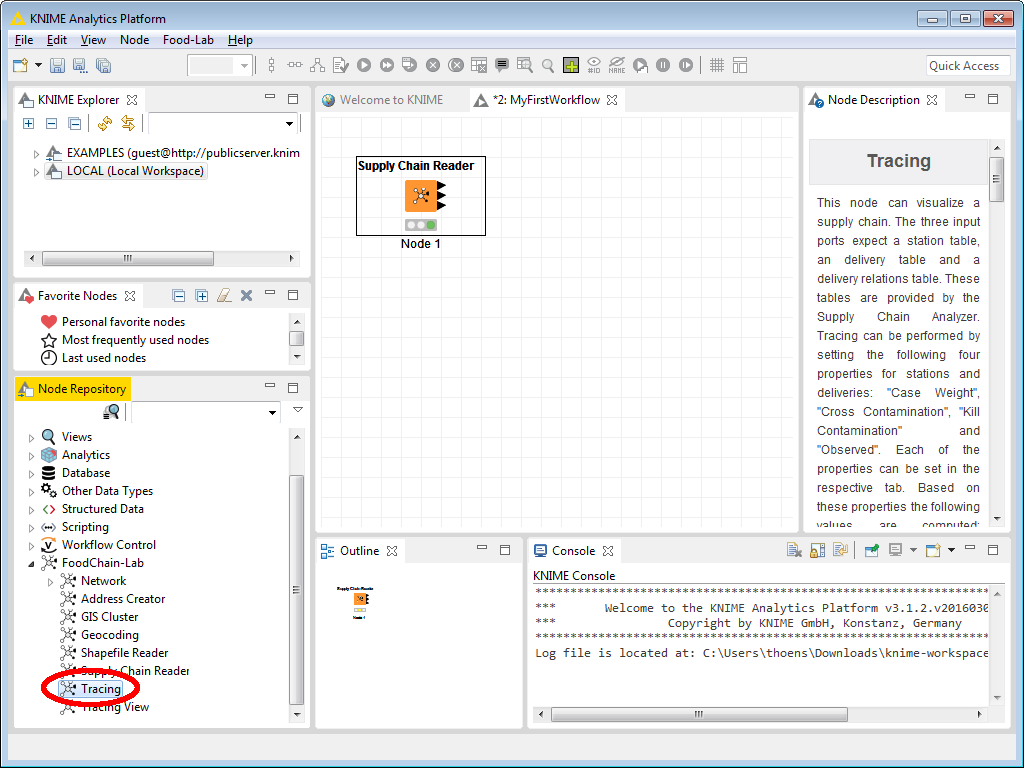
\includegraphics[height=0.6\textheight]{13.png}
	\end{center}
	\begin{itemize}
		\item The \textbf{Supply Chain Reader} has now read all data from the internal database.
		\item Select the \textbf{Supply Chain Reader} in the workflow (so that a rect is drawn around it) and double click on the \textbf{Tracing} node in the \textbf{Node Repository}.
	\end{itemize}
\end{frame}

\subsection{14}
\begin{frame}
	\begin{center}
  		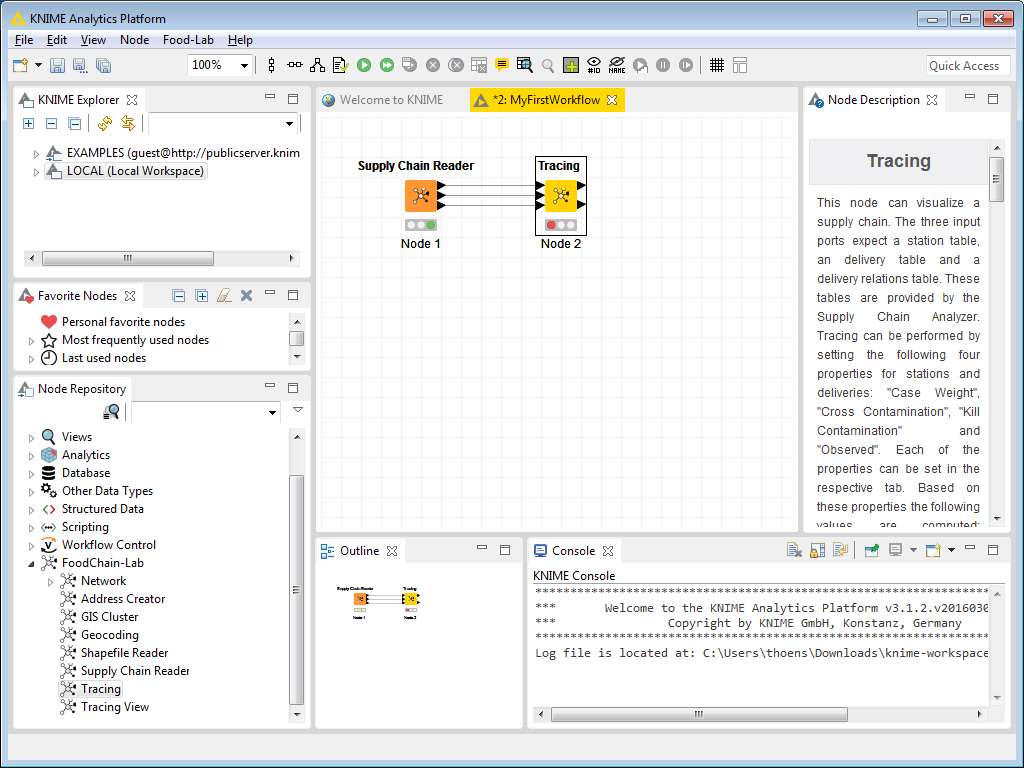
\includegraphics[height=0.6\textheight]{14.png}
	\end{center}
	\begin{itemize}
		\item The \textbf{Tracing} node should show up in the workflow and its three input ports should be automatically connected to the \textbf{Supply Chain Reader}.
		\item Double click on the \textbf{Tracing} node to configure it.
	\end{itemize}
\end{frame}

\subsection{15}
\begin{frame}
	\begin{center}
  		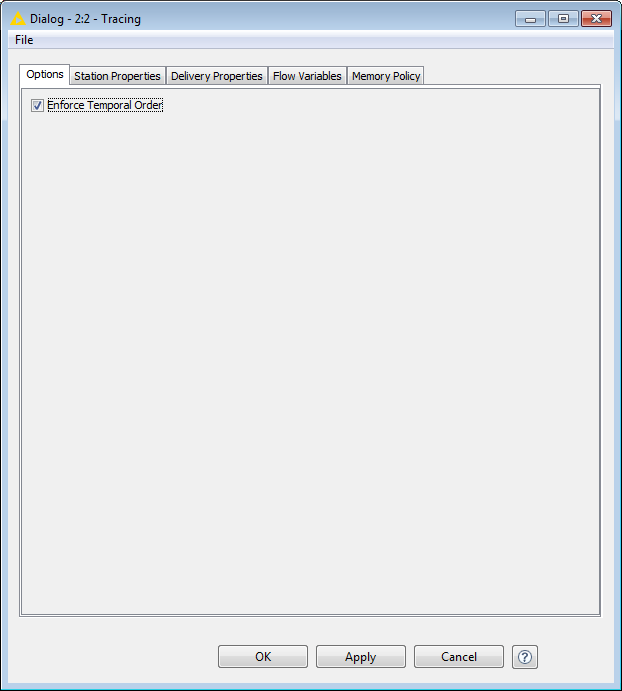
\includegraphics[height=0.5\textheight]{15.png}
	\end{center}
	\begin{itemize}
		\item You will notice tabs for "Station/Delivery Properties".
		\item "Weight", "Cross Contamination" and "Kill Contamination" can be set there. Based on these properties a "Score" is computed for each station/delivery.
		\item Additionally you can set "Observed" stations/deliveries.
		\item Select the \textbf{Station Properties} and \textbf{Weight}.
	\end{itemize}
\end{frame}

\subsection{16}
\begin{frame}
	\begin{center}
  		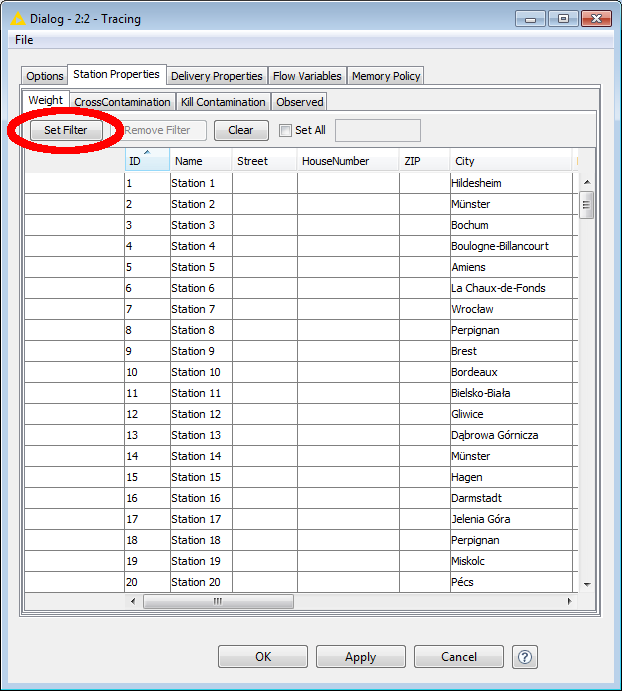
\includegraphics[height=0.6\textheight]{16.png}
	\end{center}
	\begin{itemize}
		\item A table with all available stations will show up.
		\item The weight can be set in the left column.
		\item Since scrolling through all stations is very inefficient, we can filter out all desired stations.
		\item Click on \textbf{Set Filter}.
	\end{itemize}
\end{frame}

\subsection{17}
\begin{frame}
	\begin{center}
  		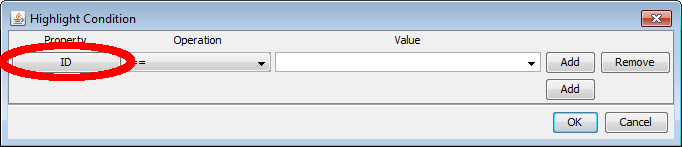
\includegraphics[width=0.9\textwidth]{17.png}
	\end{center}
	\begin{itemize}
		\item In this dialog you can specify which stations should appear in the table.
		\item Press the button in the red circle to change the value for \textbf{Property}.
	\end{itemize}
\end{frame}

\subsection{18}
\begin{frame}
	\begin{center}
  		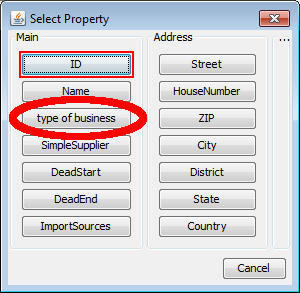
\includegraphics[width=0.4\textwidth]{18.png}
	\end{center}
	\begin{itemize}
		\item Select "type of business".
	\end{itemize}
\end{frame}

\subsection{19}
\begin{frame}
	\begin{center}
  		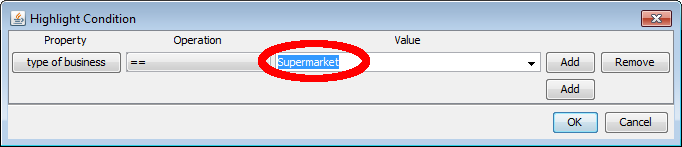
\includegraphics[width=0.7\textwidth]{19.png}
	\end{center}
	\begin{itemize}
		\item We only want to specify weights for supermarkets, since that is where contaminated products were found.
		\item Set \textbf{Value} to "Supermarket" and press \textbf{OK}.
	\end{itemize}
\end{frame}

\subsection{20}
\begin{frame}
	\begin{center}
  		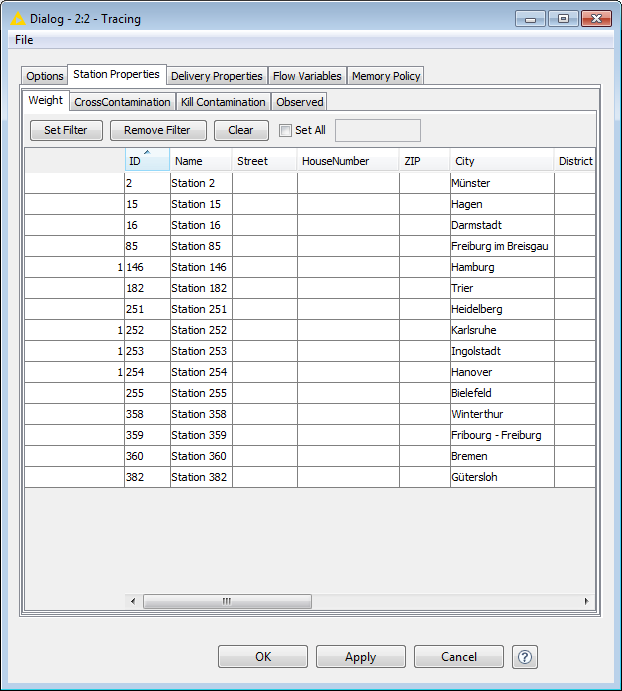
\includegraphics[height=0.6\textheight]{20.png}
	\end{center}
	\begin{itemize}
		\item Now you only see supermarkets in the dialog.
		\item Set a weight of "1" to the supermarkets in "Hamburg", "Karlsruhe", "Ingolstadt" und "Hanover" to indicate that contaminated products were found there.
		\item Click \textbf{OK} to apply the settings and close the dialog.
	\end{itemize}
\end{frame}

\subsection{21}
\begin{frame}
	\begin{center}
  		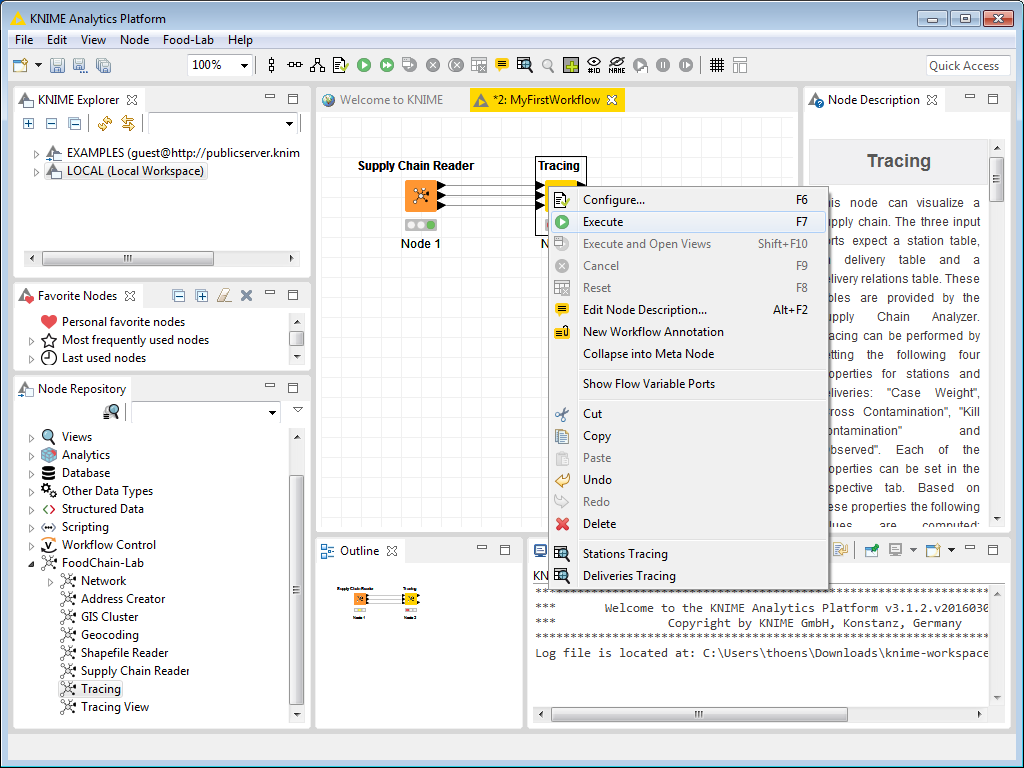
\includegraphics[height=0.6\textheight]{21.png}
	\end{center}
	\begin{itemize}
		\item Right click on the \textbf{Tracing} node and select \textbf{Execute} to execute the node.
	\end{itemize}
\end{frame}

\subsection{22}
\begin{frame}
	\begin{center}
  		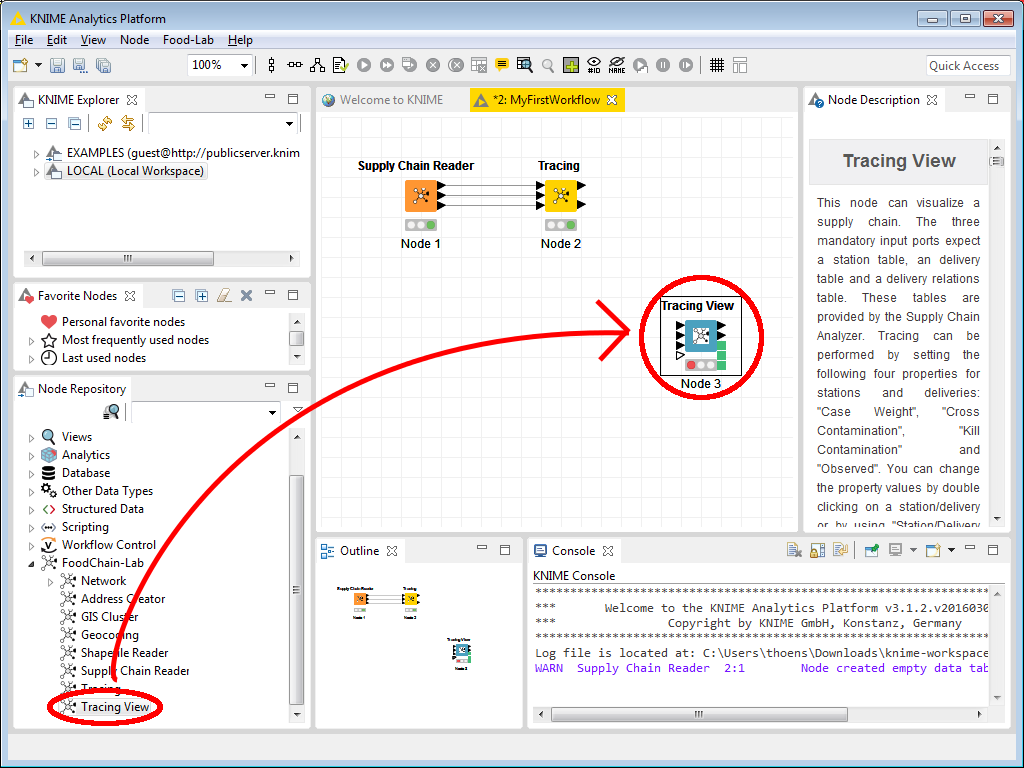
\includegraphics[height=0.6\textheight]{22.png}
	\end{center}
	\begin{itemize}
		\item Drag the \textbf{Tracing View} from the \textbf{Node Repository} to the workflow.
	\end{itemize}
\end{frame}

\subsection{23}
\begin{frame}
	\begin{center}
  		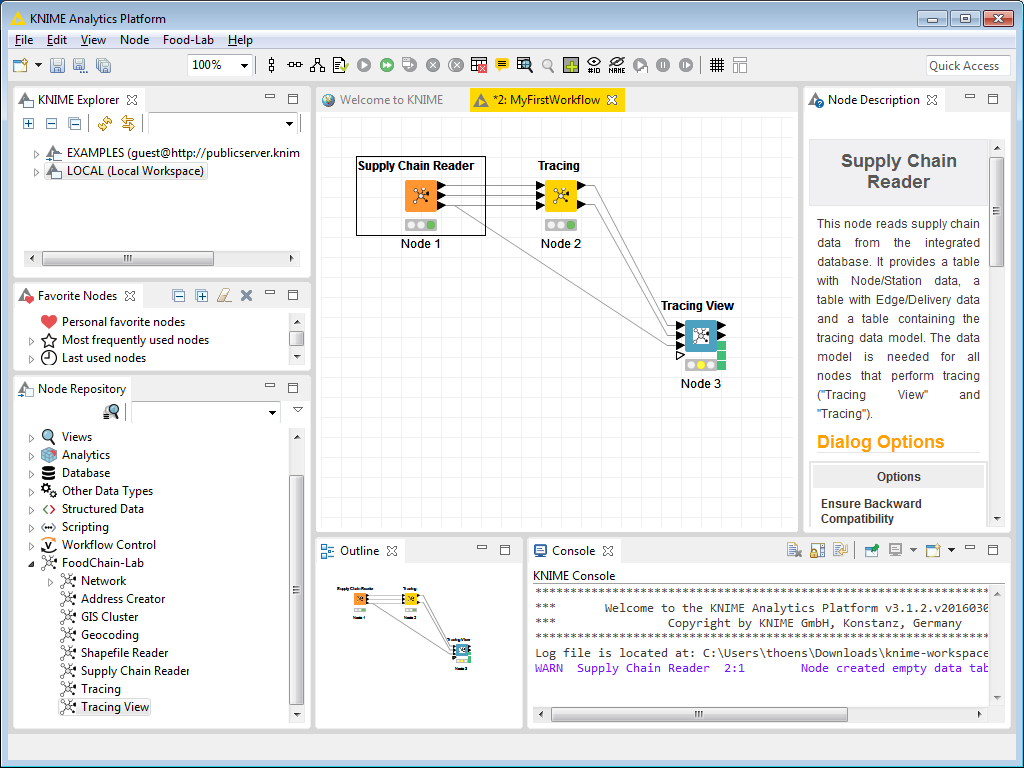
\includegraphics[height=0.6\textheight]{23.png}
	\end{center}
	\begin{itemize}
		\item Connect the output ports of the \textbf{Tracing} node to the first two input ports of the \textbf{Tracing View}.
		\item Connect the third output port of the \textbf{Supply Chain Reader} to the third input port of the \textbf{Tracing View}.
		\item Now you open the \textbf{Tracing View} and analyze the data. This will be shown in the second part of this tutorial.
	\end{itemize}
\end{frame}

\section{2-1}
\begin{frame}
	\begin{center}
  		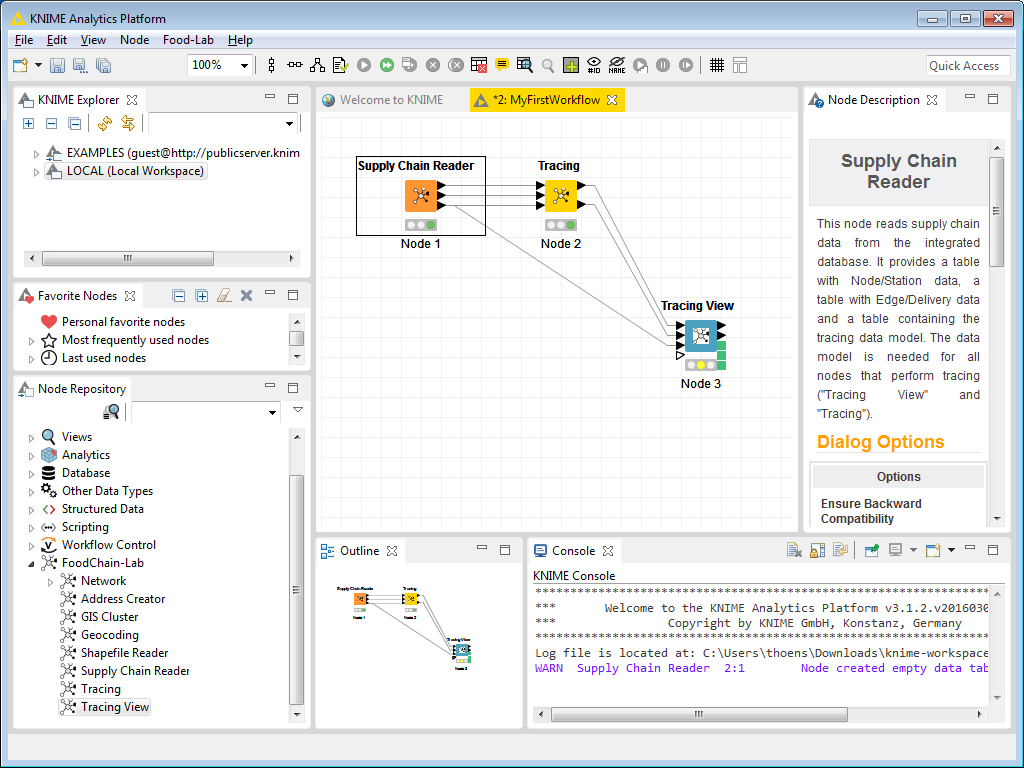
\includegraphics[height=0.6\textheight]{2-1.png}
	\end{center}
	\begin{itemize}
		\item This is the second part of the tutorial.
		\item You can either do the first part to create this workflow or download it from \url{https://github.com/SiLeBAT/BfROpenLabResources/raw/master/GitHubPages/workflows/MyFirstWorkflow.zip}.
		\item Double click on the \textbf{Tracing View} to open its dialog.
	\end{itemize}
\end{frame}

\section{2-2}
\begin{frame}
	\begin{center}
  		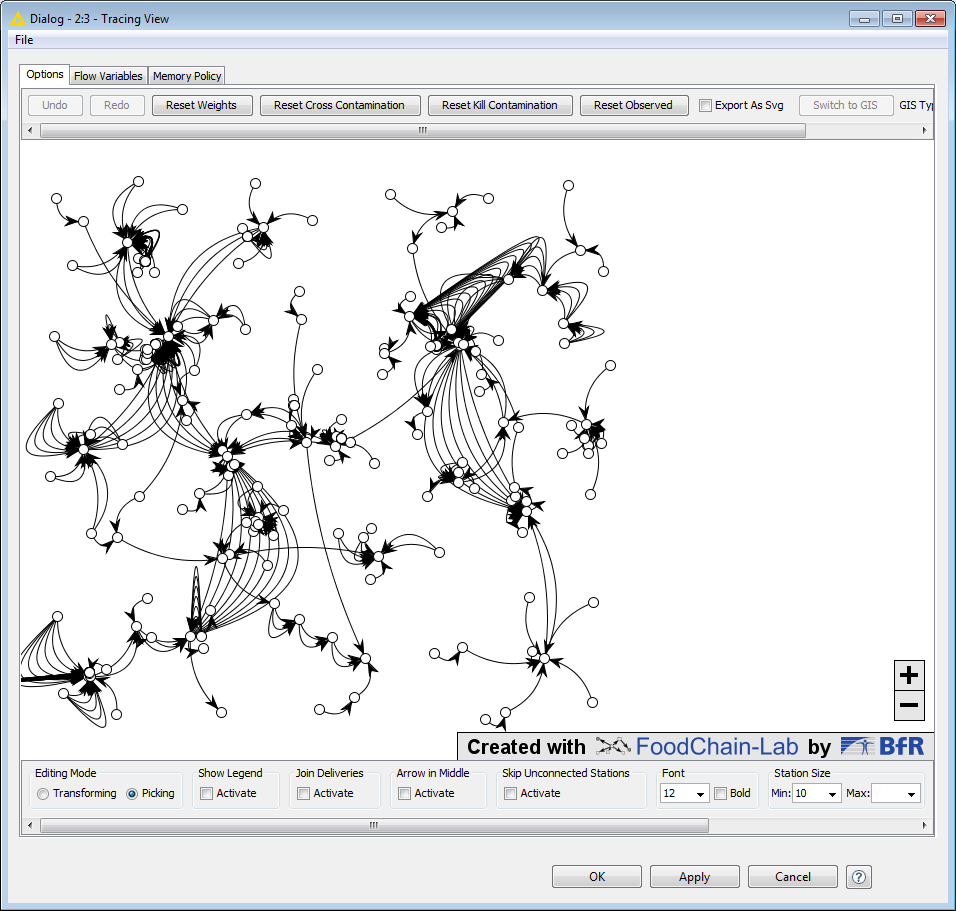
\includegraphics[height=0.6\textheight]{2-2.png}
	\end{center}
	\begin{itemize}
		\item In the \textbf{Tracing View} you can see the imported delivery network.
	\end{itemize}
\end{frame}

\section{2-3}
\begin{frame}
	\begin{center}
  		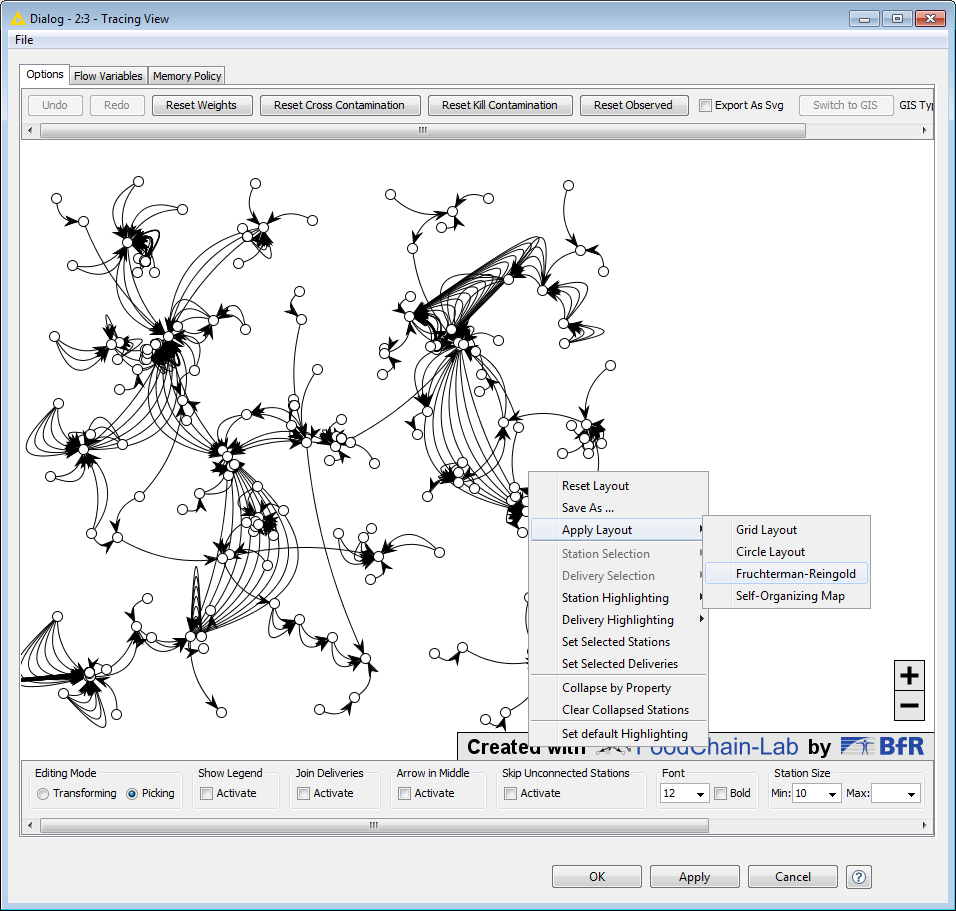
\includegraphics[height=0.6\textheight]{2-3.png}
	\end{center}
	\begin{itemize}
		\item To arrange the network in a better way right click in the graph and select \textbf{Apply Layout $>$ Fruchterman-Reingold}.
	\end{itemize}
\end{frame}

\section{2-4}
\begin{frame}
	\begin{center}
  		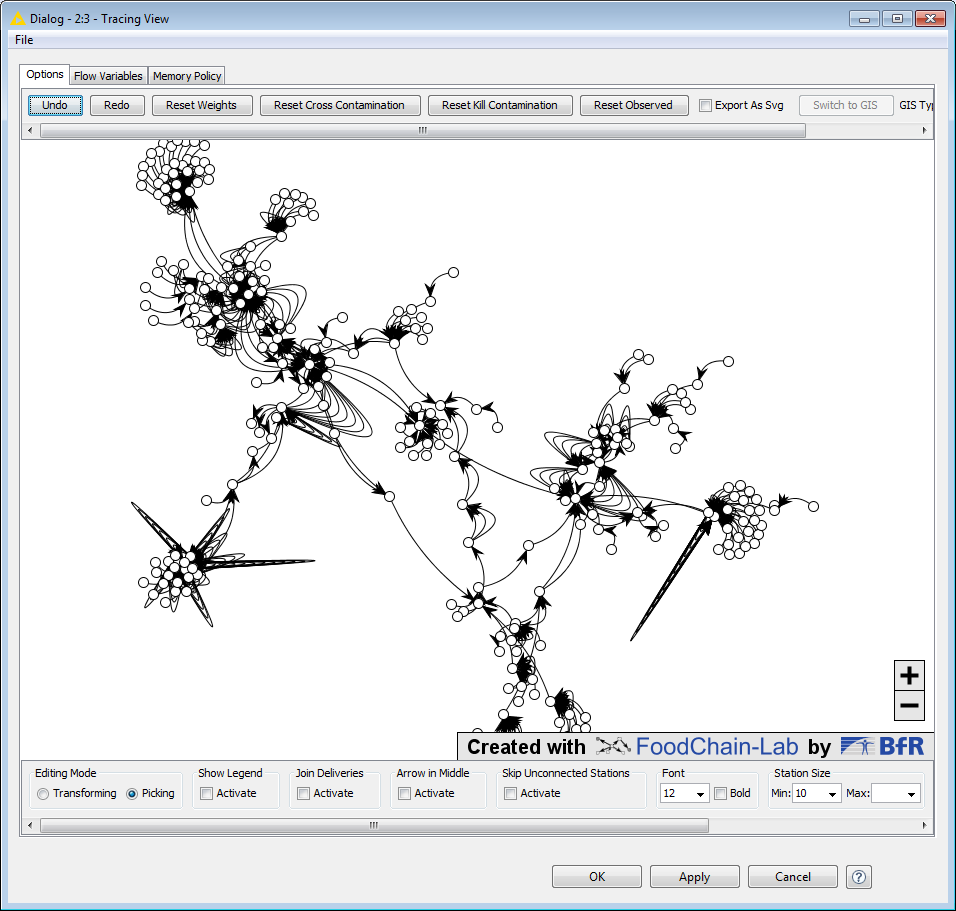
\includegraphics[height=0.55\textheight]{2-4.png}
	\end{center}
	\begin{itemize}
		\item This layout process is not deterministic. That means you will get a different result each time.
		\item You can apply the layout again, if you are not satisfied with the current result.
		\item You can also apply a layout for certain stations only. Therefore you have to select the stations you want to be layouted and apply the layout again.
	\end{itemize}
\end{frame}

\section{2-5}
\begin{frame}
	\begin{center}
  		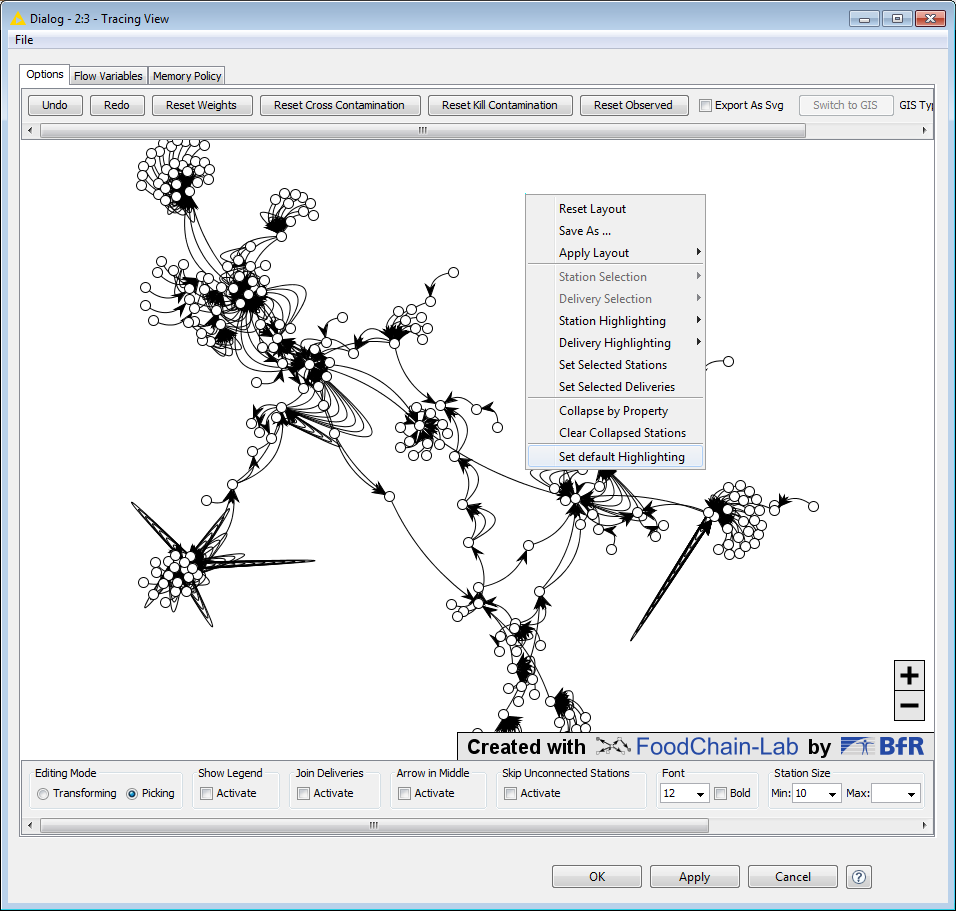
\includegraphics[height=0.6\textheight]{2-5.png}
	\end{center}
	\begin{itemize}
		\item Right click in the graph to open the context menu and select \textbf{Set default Highlighting}.
		\item Highlighting uses colors and sizes to visualize certain properties of stations/deliveries.
	\end{itemize}
\end{frame}

\section{2-6}
\begin{frame}
	\begin{center}
  		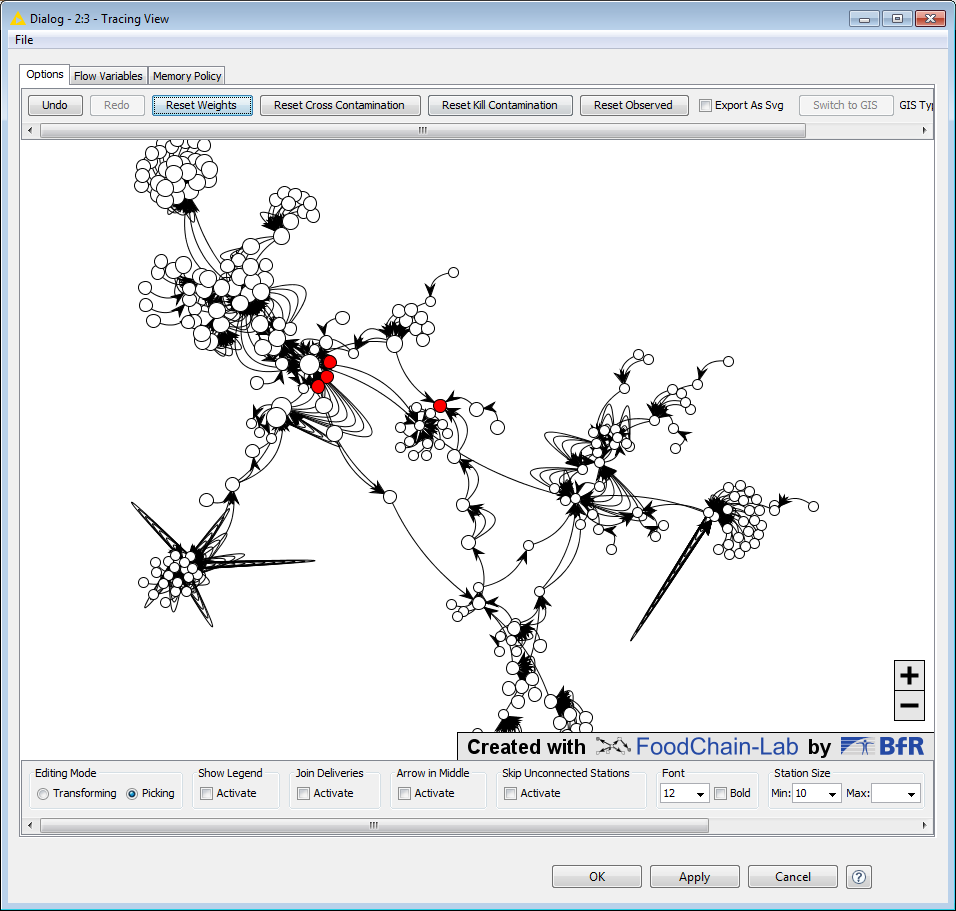
\includegraphics[height=0.6\textheight]{2-6.png}
	\end{center}
	\begin{itemize}
		\item You will notice, that 4 stations are colored red now and some stations increased in size.
		\item The red stations are the supermarkets, where we set the weight to "1".
		\item The size of each station is based on its "Score".
	\end{itemize}
\end{frame}

\section{2-7}
\begin{frame}
	\begin{center}
  		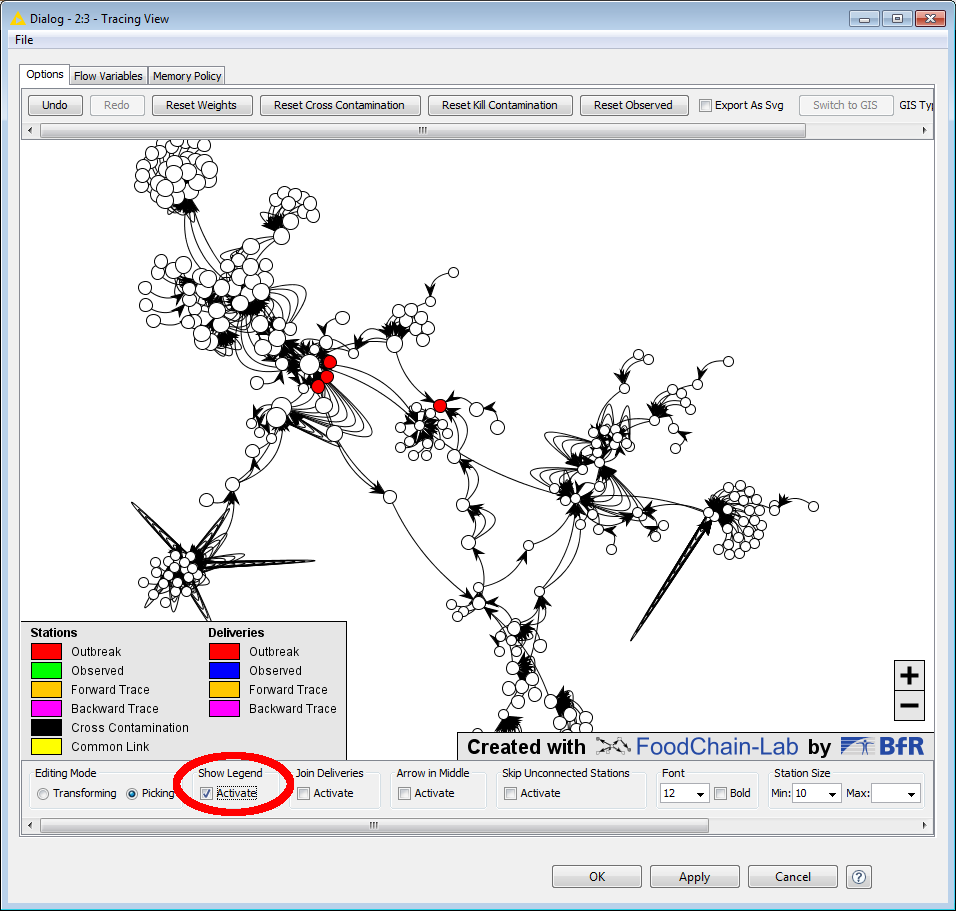
\includegraphics[height=0.6\textheight]{2-7.png}
	\end{center}
	\begin{itemize}
		\item Activate \textbf{Show Legend} to get a legend for the defined colors.
	\end{itemize}
\end{frame}

\section{2-8}
\begin{frame}
	\begin{center}
  		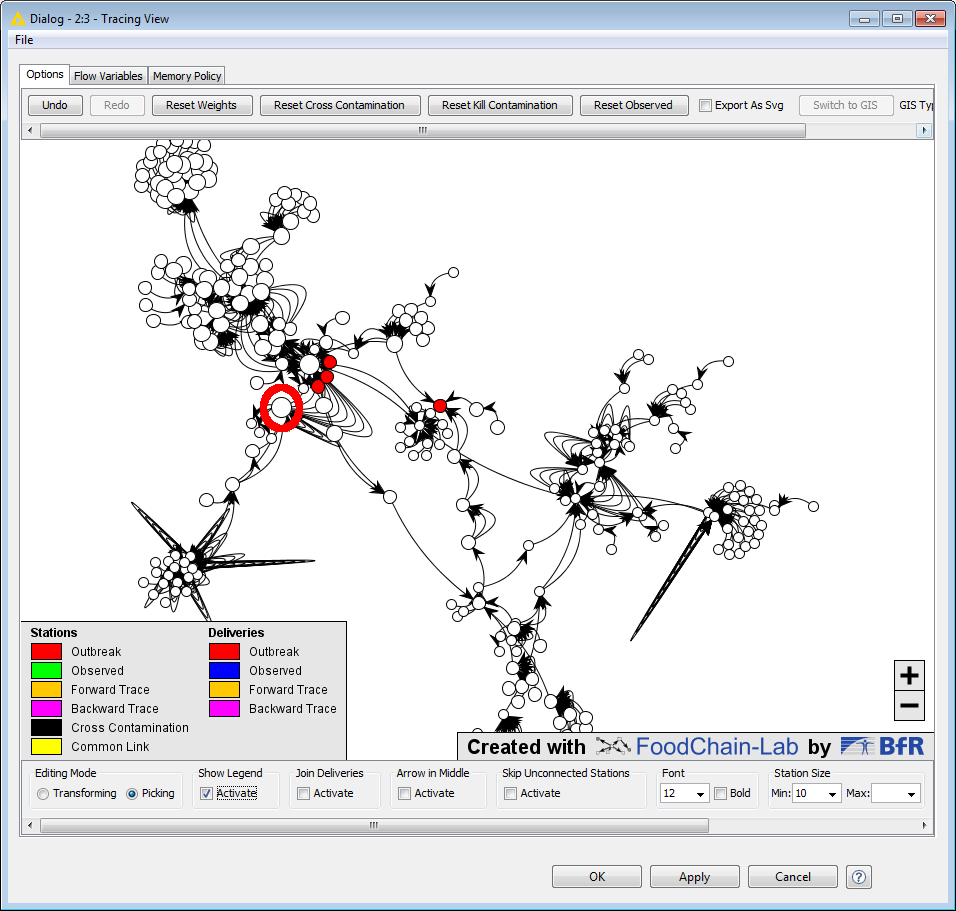
\includegraphics[height=0.6\textheight]{2-8.png}
	\end{center}
	\begin{itemize}
		\item Now we can observe a station to see its delivery trace.
		\item Set "Picking" as \textbf{Editing Mode} and double click on any station.
		\item We clicked on the station in the red circle.
	\end{itemize}
\end{frame}

\section{2-9}
\begin{frame}
	\begin{center}
  		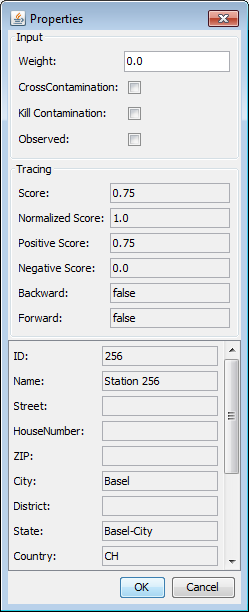
\includegraphics[height=0.6\textheight]{2-9.png}
	\end{center}
	\begin{itemize}
		\item A dialog will pop up, that shows all attributes of the station.
		\item Additionally you can change "Weight", "Cross Contamination", "Kill Contamination" and "Observed".
	\end{itemize}
\end{frame}

\section{2-10}
\begin{frame}
	\begin{center}
  		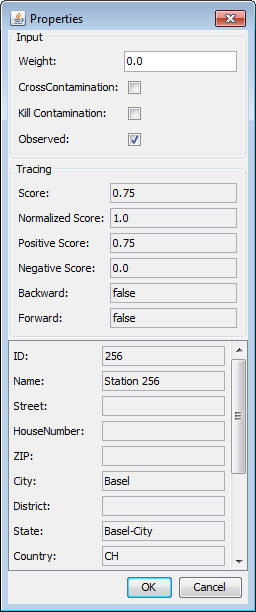
\includegraphics[height=0.6\textheight]{2-10.png}
	\end{center}
	\begin{itemize}
		\item Select \textbf{Observed} and press \textbf{OK}.
	\end{itemize}
\end{frame}

\section{2-11}
\begin{frame}
	\begin{center}
  		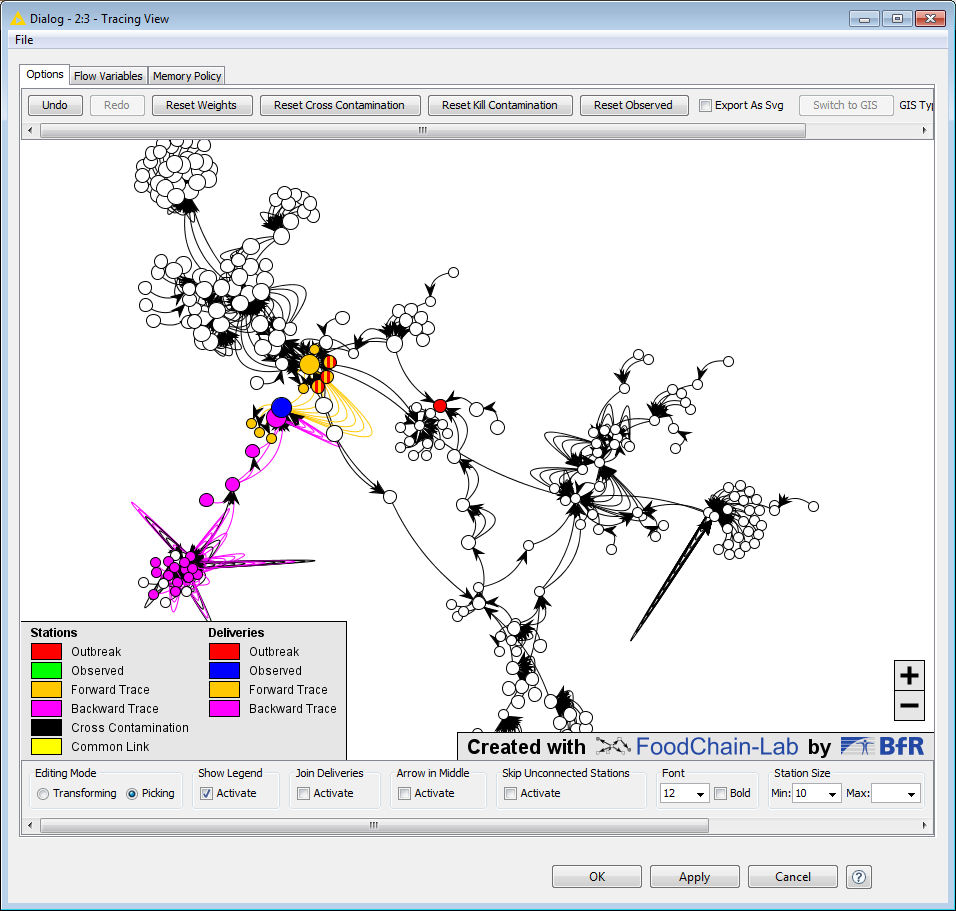
\includegraphics[height=0.6\textheight]{2-11.png}
	\end{center}
	\begin{itemize}
		\item All stations/deliveries of the forward trace are orange-colored and the ones of the backward trace are purple.
	\end{itemize}
\end{frame}

\section{2-12}
\begin{frame}
	\begin{center}
  		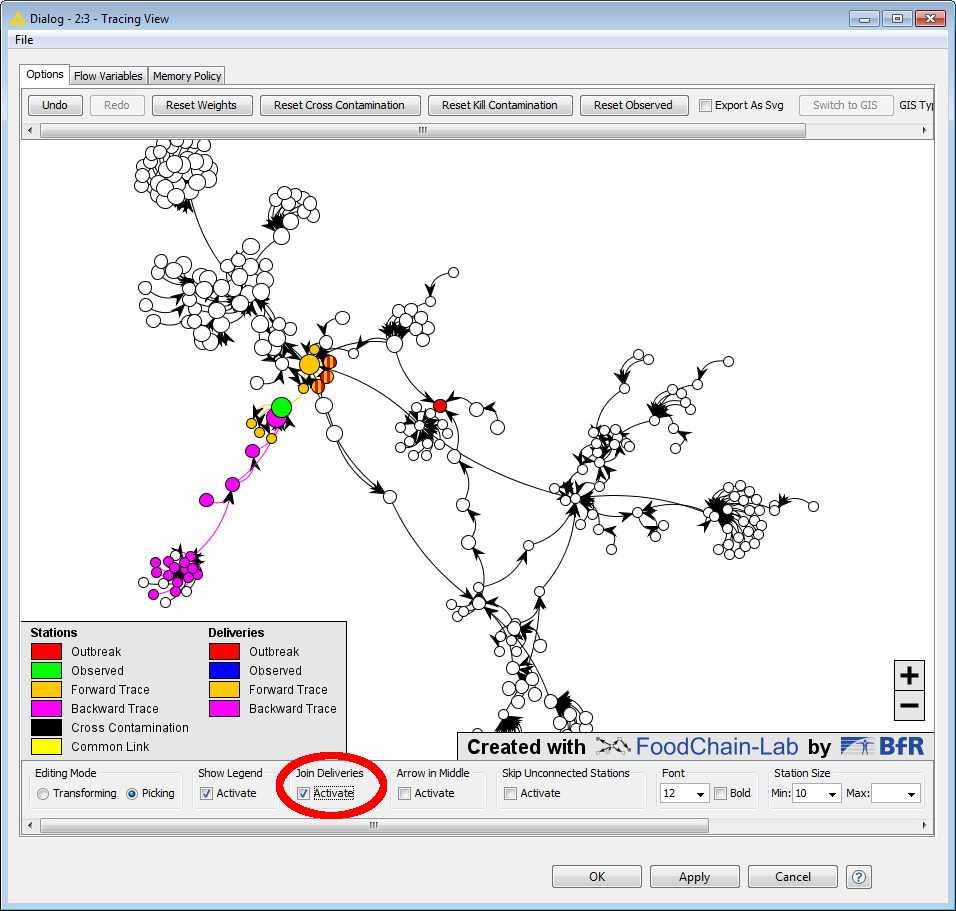
\includegraphics[height=0.6\textheight]{2-12.png}
	\end{center}
	\begin{itemize}
		\item Click at an empty area of the graph to deselect all stations.
		\item Now you can see, that the "Observed" station is green.
		\item Then activate "Join Deliveries" to simplify the graph. Deliveries with the same supplier and recipient are joined now.
	\end{itemize}
\end{frame}

\end{document}
